% !TEX root = ../BeamerTemplate.tex
%%%%%%%%%%%%%%%%%%%%%%%%%%%%%%%%%%%%%%%%%%%%%%%%%%%%%%%%%%%%%%%%%%%%%%%%%%%%%%%%%%

\section{Sionna-RT \texorpdfstring{$3\times3$}{3x3} MIMO Simulation}

\subsection{Simulation Setup}

\begin{frame}[t,shrink=8]{Sionna-RT Simulation Objective}
    \begin{columns}[T,onlytextwidth]
        \begin{column}{0.54\textwidth}
            \begin{block}{Objective}
                Evaluate how the antenna lens changes a $3\times3$ indoor
                MIMO channel at 38~GHz using Sionna-RT ray tracing.
            \end{block}

            \begin{itemize}
                \item Three TX directions: $+45^\circ$, $0^\circ$, and
                $-45^\circ$.
                \item Three RX radiation patterns represent the corresponding
                lens observation angles.
                \item With-lens and without-lens channels use identical
                propagation geometry.
            \end{itemize}
        \end{column}
        \begin{column}{0.42\textwidth}
            \begin{alertblock}{Implementation constraint}
                Sionna-RT cannot assign a different RX radiation pattern to
                each RX within the required single run.
            \end{alertblock}
            \begin{exampleblock}{Solution}
                Run three separate $3$TX-to-$1$RX simulations and combine
                their complex responses into one $3\times3$ channel matrix.
            \end{exampleblock}
        \end{column}
    \end{columns}
\end{frame}

\begin{frame}[t]{Indoor Simulation Environment: Overall View}
    \centering
    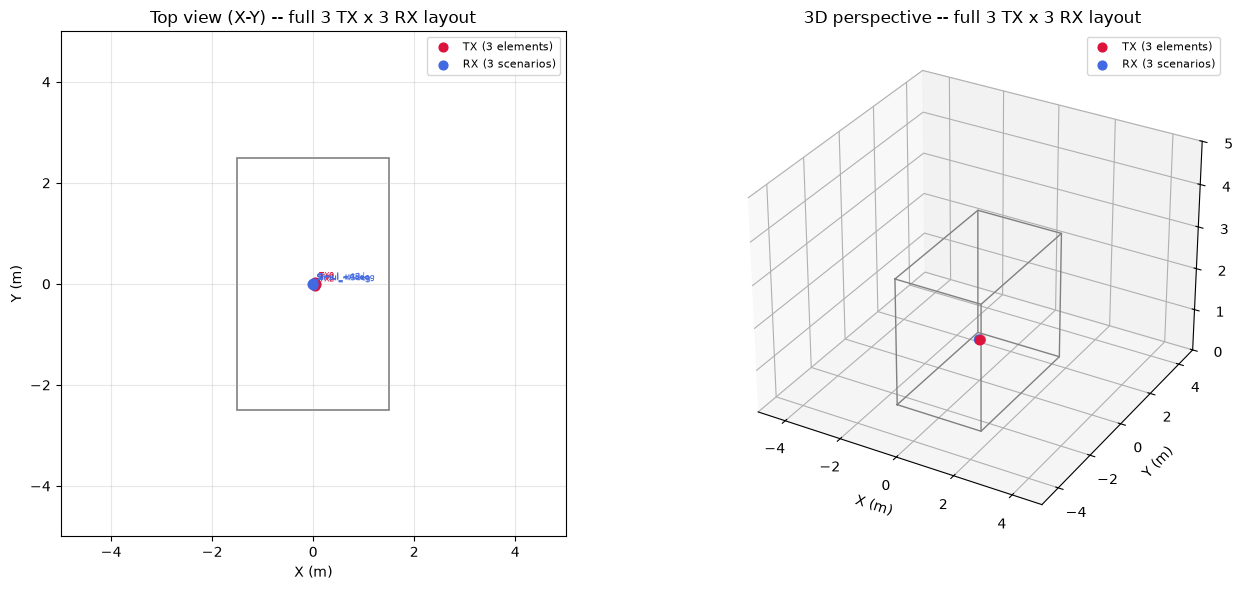
\includegraphics[width=\textwidth,height=0.62\textheight,keepaspectratio]
        {../current_report/image/SionnaSim_TotalView.png}

    \vspace{1mm}
    \begin{block}{Environment configuration}
        \centering
        \small
        Room: $3\times5\times3$~m
        \quad $\vert$ \quad
        Concrete wall: 0.2~m
        \quad $\vert$ \quad
        RX: room center
    \end{block}
\end{frame}

\begin{frame}[t]{Indoor Simulation Environment: Detailed View}
    \centering
    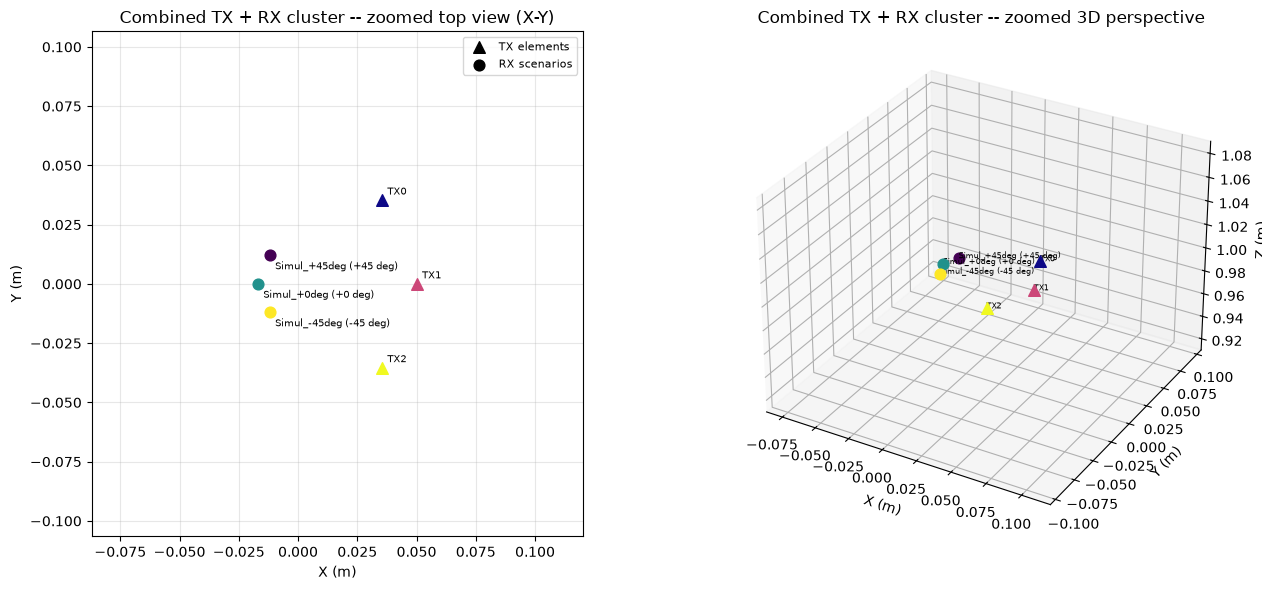
\includegraphics[width=\textwidth,height=0.59\textheight,keepaspectratio]
        {../current_report/image/SionnaSim_ZoomView.png}

    \vspace{1mm}
    \begin{block}{Wideband channel configuration}
        \centering
        \small
        Center frequency: 38~GHz
        \quad $\vert$ \quad
        Bandwidth: 2~GHz
        \quad $\vert$ \quad
        Range: 37--39~GHz
        \quad $\vert$ \quad
        Samples: 401
    \end{block}
\end{frame}

\begin{frame}[t,shrink=20]{Indoor Simulation Environment: HFSS Hybrid Setup}
    \begin{columns}[T,onlytextwidth]
        \begin{column}{0.68\textwidth}
            \centering
            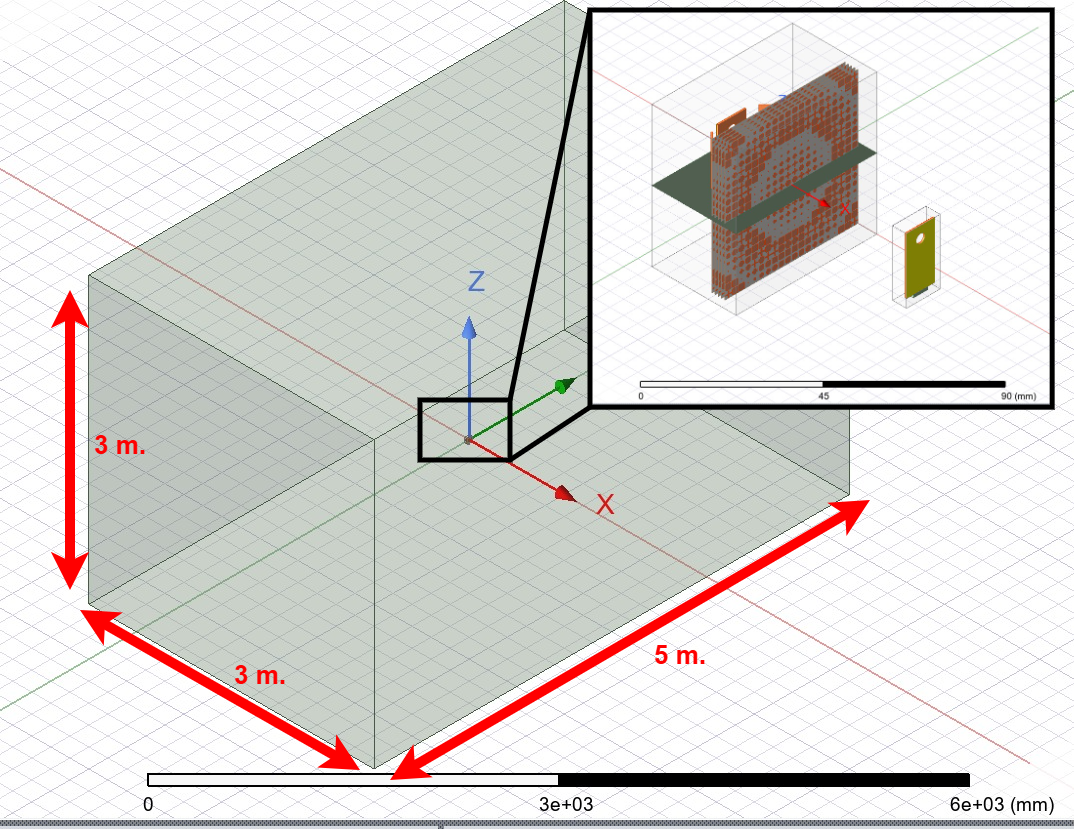
\includegraphics[width=\linewidth,height=0.55\textheight,keepaspectratio]
                {../current_report/image/Room_withCloseup.png}

            \scriptsize HFSS Hybrid room and close-up of the antenna-lens placement
        \end{column}
        \begin{column}{0.29\textwidth}
            \small
            \begin{block}{Hybrid representation}
                \begin{itemize}
                    \item One swept TX source
                    \item Three RX observation points
                    \item Incident angles:
                    $+45^\circ$, $0^\circ$, $-45^\circ$
                    \item With- and without-lens cases
                \end{itemize}
            \end{block}
            \begin{alertblock}{Same physical setup}
                The room, lens position, focal radius, and RX angular
                directions follow the same reference geometry used for the
                Sionna-RT study.
            \end{alertblock}
        \end{column}
    \end{columns}
\end{frame}

\begin{frame}[t,shrink=20]{Indoor Simulation Environment: HFSS SBR+ Setup}
    \begin{columns}[T,onlytextwidth]
        \begin{column}{0.68\textwidth}
            \centering
            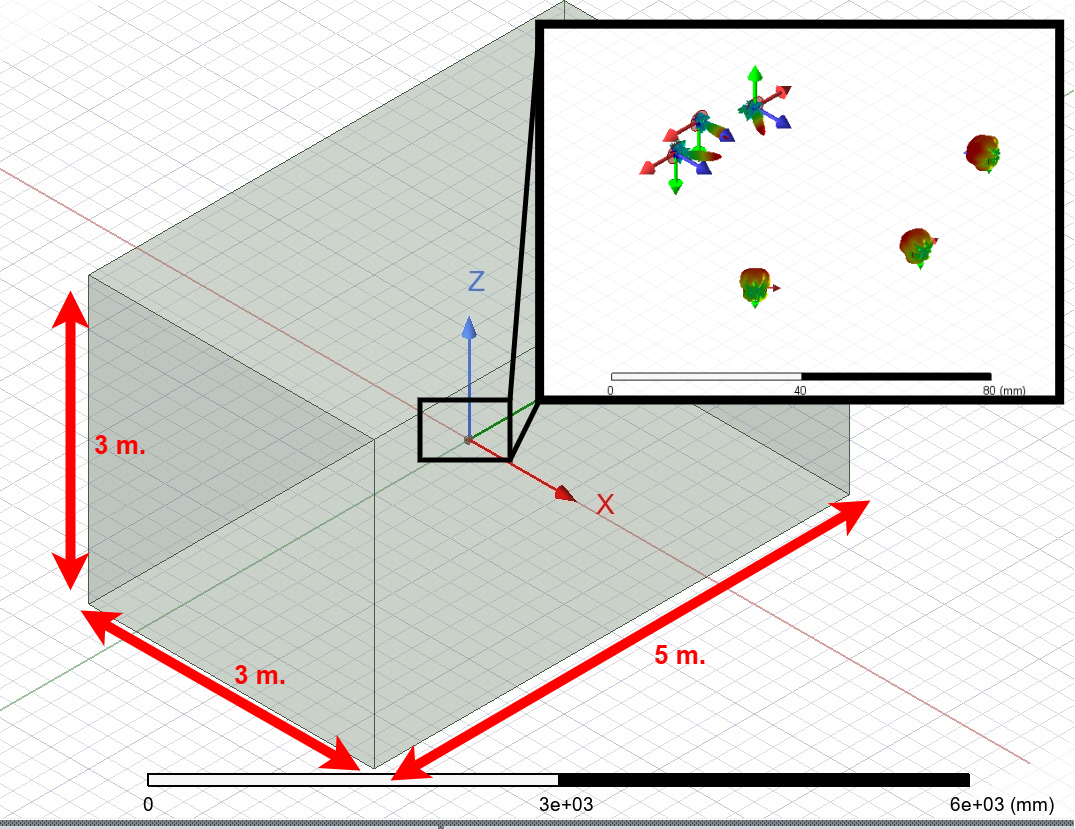
\includegraphics[width=\linewidth,height=0.55\textheight,keepaspectratio]
                {../current_report/image/Room_SBR_withCloseup.png}

            \scriptsize HFSS SBR+ room and close-up of the physical
            $3$TX-to-$3$RX arrangement
        \end{column}
        \begin{column}{0.29\textwidth}
            \small
            \begin{block}{SBR+ representation}
                \begin{itemize}
                    \item Three physical TX positions
                    \item Three RX observation points
                    \item Lens and no-lens cases
                    \item Ray-traced response at 37, 38, and 39~GHz
                \end{itemize}
            \end{block}
            \begin{alertblock}{Same physical setup}
                This is the reference geometry reproduced in Sionna-RT:
                identical room concept, TX/RX directions, lens placement,
                and focal arrangement.
            \end{alertblock}
        \end{column}
    \end{columns}
\end{frame}

\begin{frame}[t,shrink=15]{Common Experimental Setup Across the Three Solvers}
    \begin{block}{Clarification}
        \centering
        \textbf{Sionna-RT, HFSS SBR+, and HFSS Hybrid evaluate the same
        underlying indoor antenna-lens setup.}
    \end{block}

    \small
    \resizebox{\textwidth}{!}{%
    \begin{tabular}{@{}p{0.22\textwidth}p{0.22\textwidth}p{0.22\textwidth}
        p{0.26\textwidth}@{}}
        \toprule
        \textbf{Common basis} & \textbf{Sionna-RT} & \textbf{HFSS SBR+} &
        \textbf{HFSS Hybrid} \\
        \midrule
        $3\times5\times3$~m room, 0.2-m concrete walls, centered lens,
        three angular directions, and with/without-lens comparison
        &
        Three $3$TX-to-$1$RX runs are combined into a $3\times3$ channel
        &
        Physical $3$TX-to-$3$RX ray-tracing model
        &
        One TX is swept over three incident angles and observed at three RX
        points \\
        \bottomrule
    \end{tabular}
    }

    \vspace{3mm}
    \begin{exampleblock}{Interpretation}
        Differences among the figures reflect solver-specific modeling and
        execution strategies; they do \emph{not} represent different physical
        room scenarios.
    \end{exampleblock}
\end{frame}

\subsection{Channel Formulation}

\begin{frame}[t,shrink=22]{Wideband Multipath Channel Model}
    \begin{columns}[T,onlytextwidth]
        \begin{column}{0.53\textwidth}
            \begin{block}{Frequency response}
                \[
                    H(f)=\frac{V_{\mathrm R}}{V_{\mathrm T}}
                    =\sum_{i=1}^{N}\alpha_i e^{-j2\pi f\tau_i}
                \]
                \small
                Each path coefficient $\alpha_i$ contains spreading,
                material interaction, polarization, and antenna-pattern
                effects; $\tau_i=r_i/c_i$ is its delay.
            \end{block}

            \begin{block}{Complex-baseband impulse response}
                \[
                    h_{\mathrm b}(\tau)=
                    \sum_{i=1}^{N}
                    \alpha_i e^{-j2\pi f_{\mathrm c}\tau_i}
                    \delta(\tau-\tau_i)
                \]
            \end{block}
        \end{column}
        \begin{column}{0.43\textwidth}
            \begin{block}{Wideband sampling}
                \[
                    \Delta f=\frac{B}{N_f-1}
                    =\frac{2~\mathrm{GHz}}{400}
                    =5~\mathrm{MHz}
                \]
            \end{block}

            \begin{itemize}
                \item The same 401-point frequency grid is used for all three
                RX-pattern simulations.
                \item Complex magnitude and phase are retained when the
                responses are assembled into $\mathbf H(f)$.
                \item Coherent path summation captures constructive and
                destructive interference.
            \end{itemize}
        \end{column}
    \end{columns}
\end{frame}

\subsection{Channel-Magnitude Results}

\begin{frame}[t]{Channel Magnitude Across 37--39~GHz}
    \centering
    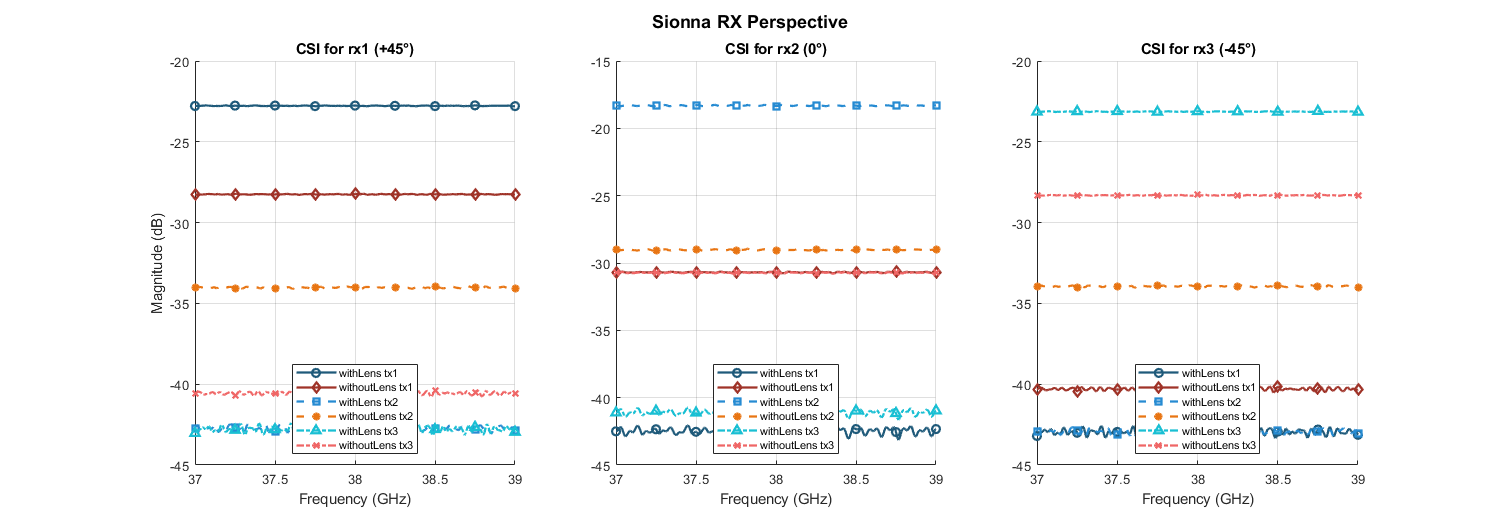
\includegraphics[width=\textwidth,height=0.72\textheight,keepaspectratio]
        {../current_report/image/Sionna_result.png}

    \vspace{-1mm}
    \begin{exampleblock}{Main observation}
        \small
        The lens strengthens each direction-matched link
        (TX1--RX1, TX2--RX2, and TX3--RX3), while several non-aligned links
        are attenuated. The response is nearly flat across the 2-GHz band.
    \end{exampleblock}
\end{frame}

\begin{frame}[t,shrink=10]{Directional Gain of the Aligned Links}
    \begin{columns}[T,onlytextwidth]
        \begin{column}{0.57\textwidth}
            \centering
            \small
            \begin{tabular}{lrrr}
                \toprule
                \textbf{Aligned link} &
                \makecell{\textbf{Lens}\\\textbf{(dB)}} &
                \makecell{\textbf{No lens}\\\textbf{(dB)}} &
                \makecell{\textbf{Gain}\\\textbf{(dB)}} \\
                \midrule
                TX1--RX1 ($+45^\circ$) & $-22.7$ & $-28.3$ & $+5.6$ \\
                TX2--RX2 ($0^\circ$)   & $-18.2$ & $-29.0$ & $+10.8$ \\
                TX3--RX3 ($-45^\circ$) & $-23.0$ & $-28.3$ & $+5.3$ \\
                \bottomrule
            \end{tabular}

            \vspace{5mm}
            \[
                \Delta H_{\mathrm{lens}}=
                H_{\mathrm{with~lens,dB}}
                -H_{\mathrm{without~lens,dB}}
            \]
        \end{column}
        \begin{column}{0.39\textwidth}
            \begin{exampleblock}{Strongest focusing}
                The boresight link TX2--RX2 gains approximately
                \textbf{10.8~dB}.
            \end{exampleblock}
            \begin{alertblock}{Angular rejection}
                For the RX2 perspective, non-aligned TX1 and TX3 are reduced
                from about $-30.5$~dB to $-42$--$-41$~dB.
            \end{alertblock}
            \small
            The lens reshapes the matrix toward dominant diagonal links
            instead of providing uniform gain.
        \end{column}
    \end{columns}
\end{frame}

\begin{frame}[t]{Lens-Induced Change in All TX--RX Links}
    \centering
    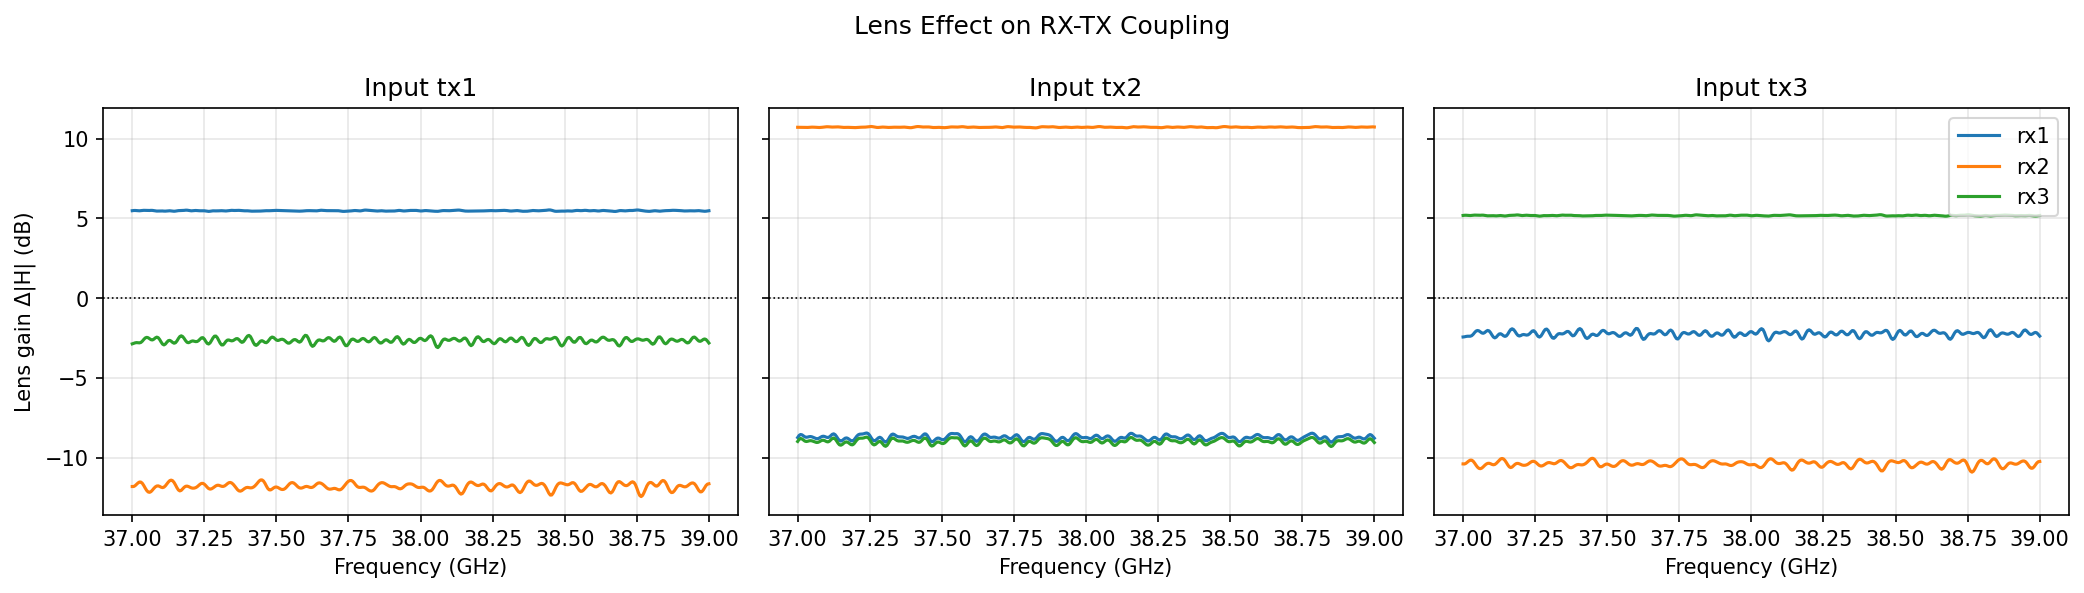
\includegraphics[width=\textwidth,height=0.70\textheight,keepaspectratio]
        {../current_report/image/sionna_lens_effect_delta.png}

    \vspace{-1mm}
    \small
    \begin{itemize}
        \item Aligned links gain approximately $+5.5$, $+10.7$, and
        $+5.1$~dB for TX1--RX1, TX2--RX2, and TX3--RX3.
        \item Most cross-directional links are attenuated by
        approximately $2.5$--$12$~dB.
    \end{itemize}
\end{frame}

\subsection{MIMO Evaluation}

\begin{frame}[t,shrink=12]{Singular Values and Channel Quality}
    \begin{columns}[T,onlytextwidth]
        \begin{column}{0.64\textwidth}
            \centering
            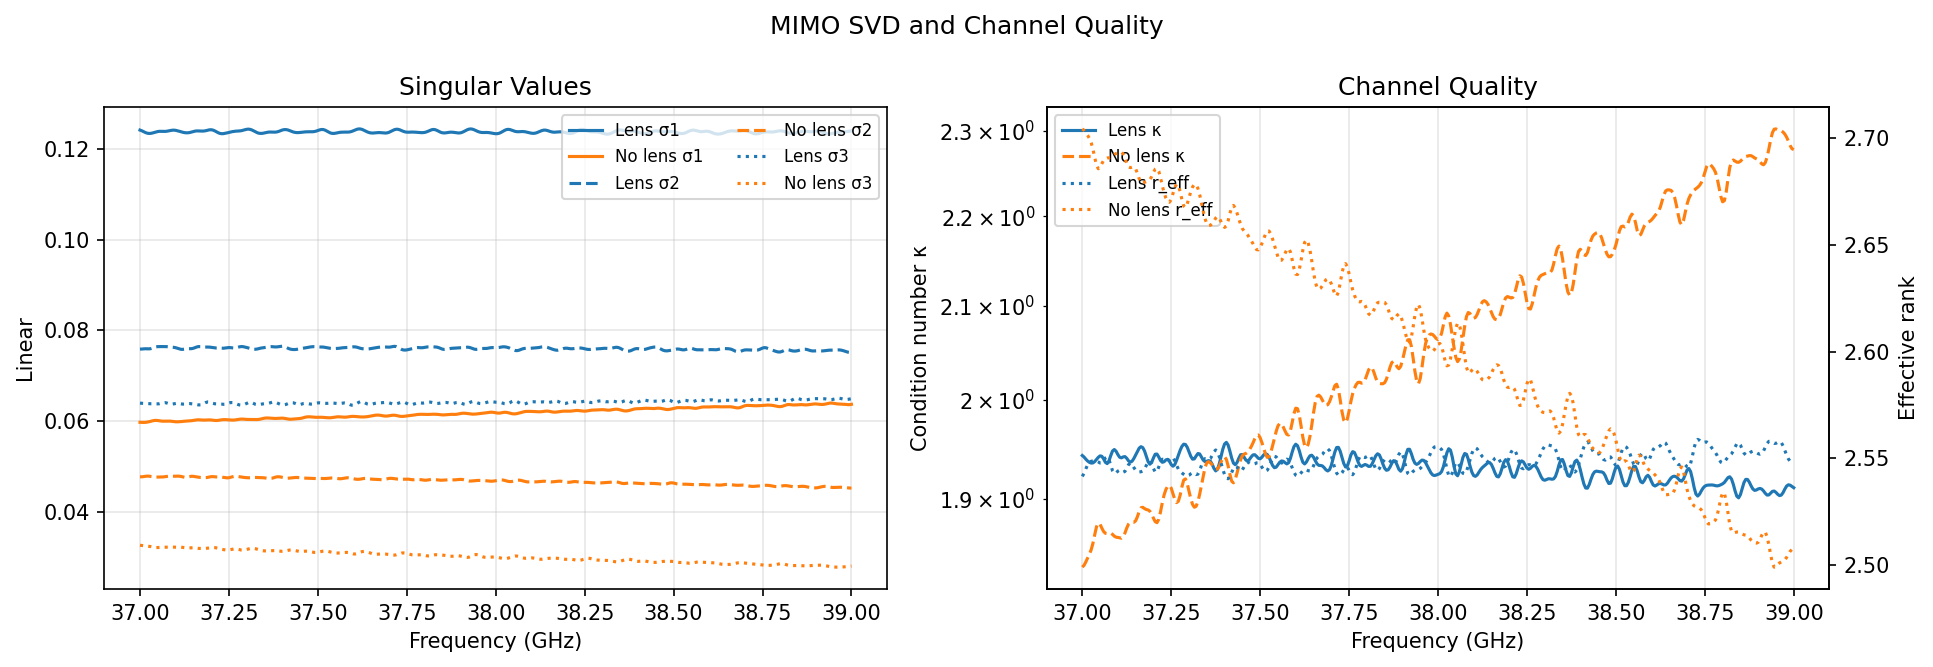
\includegraphics[width=\linewidth,height=0.72\textheight,keepaspectratio]
                {../current_report/image/sionna_mimo_quality.png}
        \end{column}
        \begin{column}{0.33\textwidth}
            \scriptsize
            \begin{block}{Mean singular values}
                \begin{tabular}{@{}lcc@{}}
                    & \textbf{Lens} & \textbf{No lens} \\
                    $\sigma_1$ & 0.1239 & 0.0618 \\
                    $\sigma_2$ & 0.0760 & 0.0467 \\
                    $\sigma_3$ & 0.0642 & 0.0300
                \end{tabular}
            \end{block}
            \begin{block}{Conditioning}
                Mean $\kappa$: 1.931 with lens versus 2.066 without lens.
                The lens result is also more stable over frequency.
            \end{block}
            \begin{alertblock}{Qualified rank result}
                Mean effective rank is 2.549 with lens and 2.603 without
                lens. The primary benefit is stronger, more stable modes,
                not a uniformly higher effective rank.
            \end{alertblock}
        \end{column}
    \end{columns}
\end{frame}

\begin{frame}[t,shrink=22]{Equal-Power MIMO Capacity}
    \begin{columns}[T,onlytextwidth]
        \begin{column}{0.64\textwidth}
            \centering
            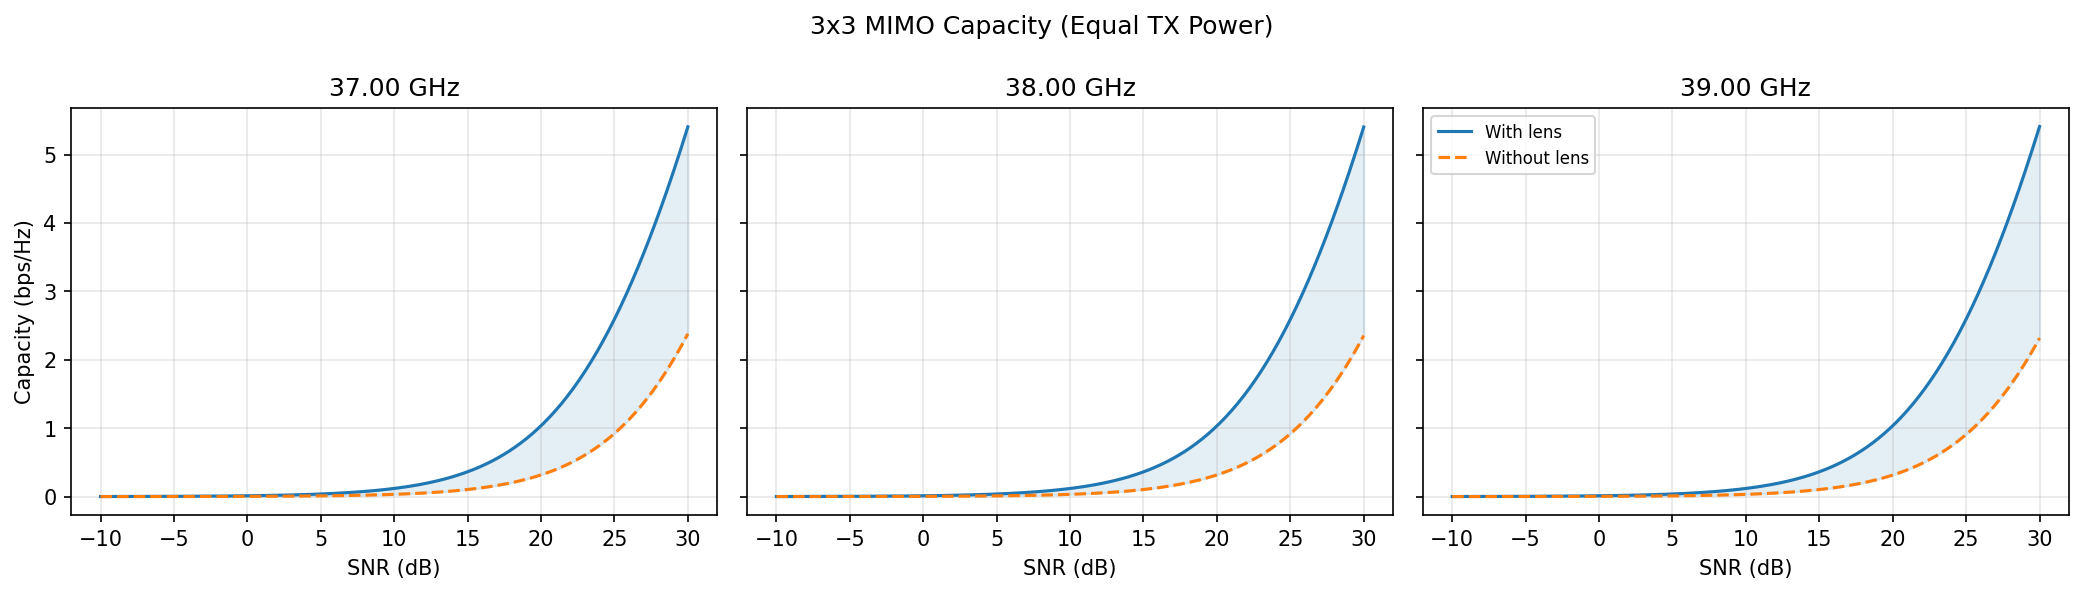
\includegraphics[width=\linewidth,height=0.70\textheight,keepaspectratio]
                {../current_report/image/sionna_mimo_capacity.png}
        \end{column}
        \begin{column}{0.33\textwidth}
            \small
            \[
                C=\log_2\det\!\left(
                \mathbf I_3+\frac{\rho}{3}
                \mathbf H\mathbf H^{H}\right)
            \]
            \begin{exampleblock}{30-dB mean capacity}
                \centering
                \textbf{With lens: 5.406~bps/Hz}\\
                Without lens: 2.351~bps/Hz
            \end{exampleblock}
            \begin{itemize}
                \item Advantage appears at 37, 38, and 39~GHz.
                \item Small inter-frequency variation confirms a broadband
                capacity benefit.
            \end{itemize}
        \end{column}
    \end{columns}
\end{frame}

\begin{frame}[t]{Capacity Stability Across Frequency}
    \begin{columns}[T,onlytextwidth]
        \begin{column}{0.66\textwidth}
            \centering
            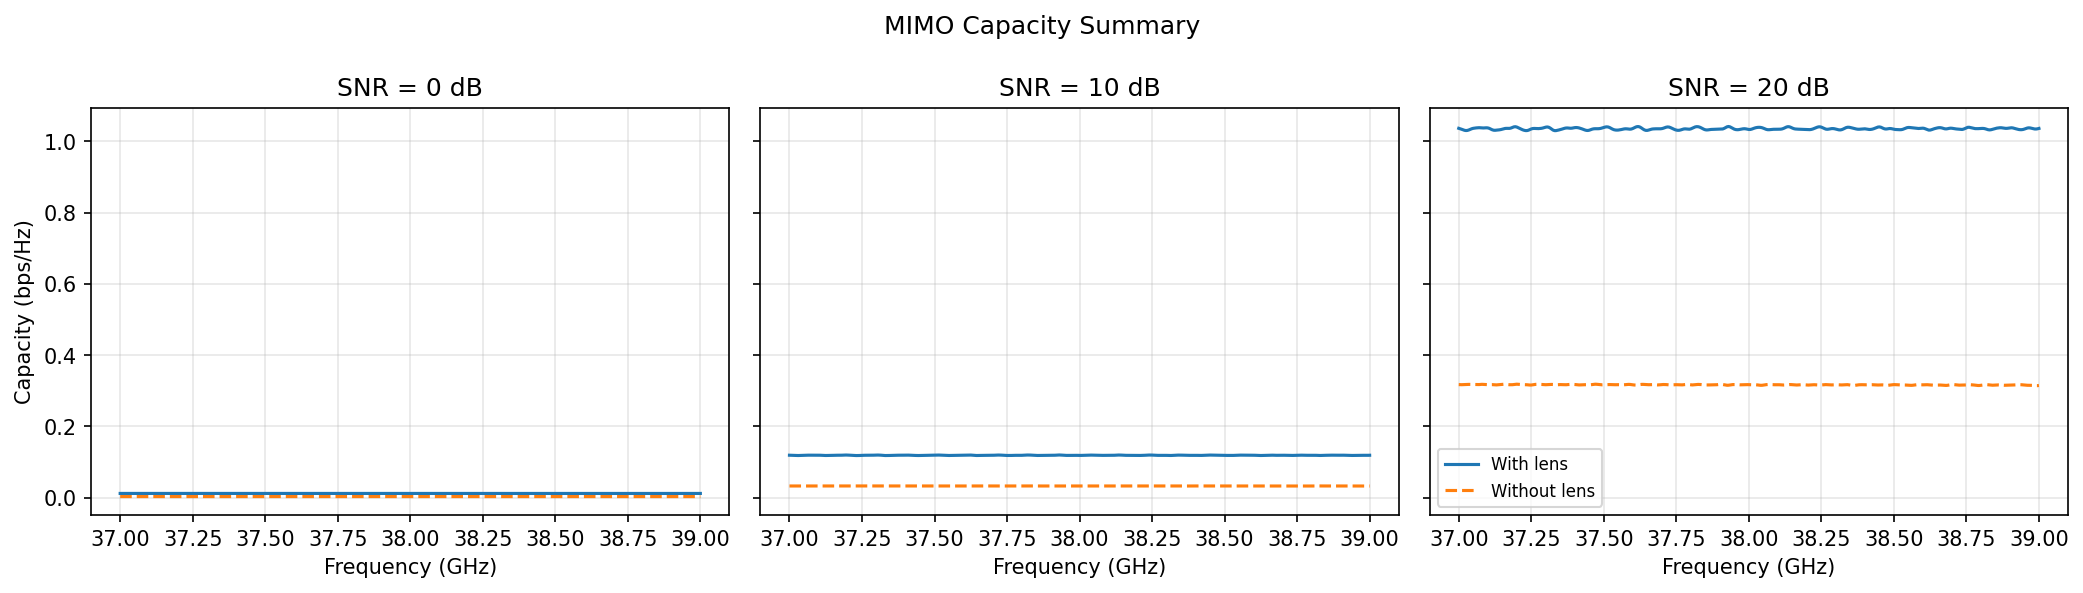
\includegraphics[width=\linewidth,height=0.72\textheight,keepaspectratio]
                {../current_report/image/sionna_mimo_capacity_summary.png}
        \end{column}
        \begin{column}{0.30\textwidth}
            \scriptsize
            \begin{block}{Full-band mean capacity}
                \begin{tabular}{@{}rcc@{}}
                    \toprule
                    \textbf{SNR} & \textbf{Lens} & \textbf{No lens} \\
                    \midrule
                    0~dB  & 0.01211 & 0.00332 \\
                    10~dB & 0.1191  & 0.03303 \\
                    20~dB & 1.0353  & 0.3169 \\
                    \bottomrule
                \end{tabular}
            \end{block}
            \begin{exampleblock}{Capacity ratio}
                Lens/no-lens ratios are approximately
                \textbf{3.65}, \textbf{3.61}, and \textbf{3.27} at
                0, 10, and 20~dB.
            \end{exampleblock}
            Results are nearly frequency-flat over 37--39~GHz.
        \end{column}
    \end{columns}
\end{frame}

\begin{frame}[t,shrink=15]{Spatial Correlation at 38~GHz}
    \begin{columns}[T,onlytextwidth]
        \begin{column}{0.65\textwidth}
            \centering
            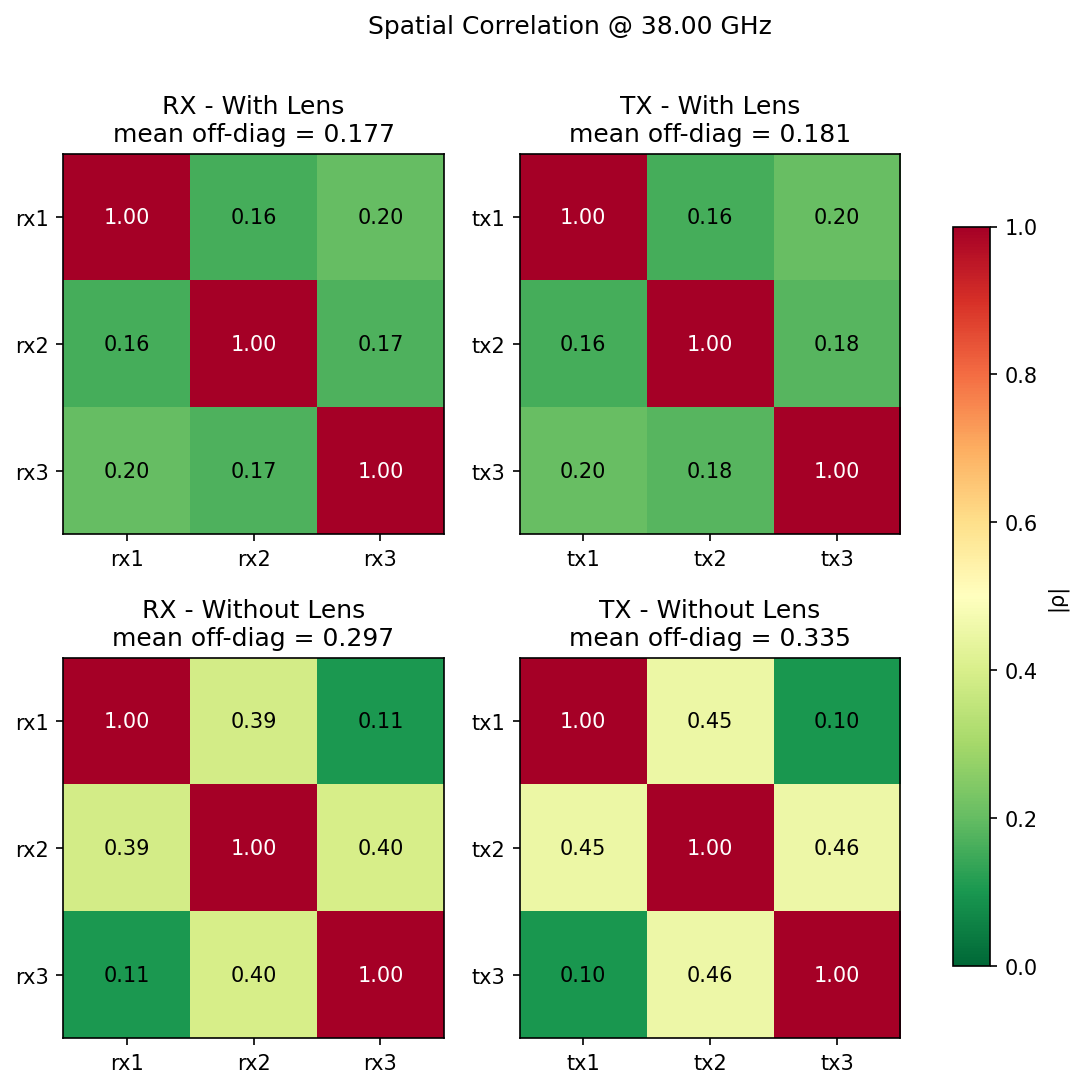
\includegraphics[width=\linewidth,height=0.72\textheight,keepaspectratio]
                {../current_report/image/sionna_spatial_correlation.png}
        \end{column}
        \begin{column}{0.31\textwidth}
            \small
            \begin{block}{Mean off-diagonal correlation}
                \begin{tabular}{@{}lcc@{}}
                    & \textbf{Lens} & \textbf{No lens} \\
                    RX & 0.177 & 0.297 \\
                    TX & 0.181 & 0.335
                \end{tabular}
            \end{block}
            \begin{exampleblock}{Reduction}
                RX correlation decreases by \textbf{40.4\%}; TX correlation
                decreases by \textbf{46.0\%}.
            \end{exampleblock}
            Lower off-diagonal correlation indicates better separation among
            TX and RX channel vectors.
        \end{column}
    \end{columns}
\end{frame}

\subsection{Conclusions}

\begin{frame}[t,shrink=8]{Sionna-RT Conclusions}
    \begin{columns}[T,onlytextwidth]
        \begin{column}{0.49\textwidth}
            \begin{exampleblock}{What the lens improves}
                \begin{itemize}
                    \item Strengthens all three direction-matched links.
                    \item Suppresses most cross-directional coupling.
                    \item Increases all three singular-mode strengths.
                    \item Provides stable conditioning and capacity over
                    37--39~GHz.
                    \item Reduces RX- and TX-side spatial correlation.
                \end{itemize}
            \end{exampleblock}
        \end{column}
        \begin{column}{0.47\textwidth}
            \begin{alertblock}{Important qualification}
                The lens does not provide uniform gain and does not increase
                effective rank at every frequency.
            \end{alertblock}

            \begin{block}{Engineering interpretation}
                Directional focusing translates into a
                \textbf{stronger and more separable $3\times3$ channel}.
                The main advantage comes from stronger, more frequency-stable
                eigenchannels rather than from creating additional spatial
                modes.
            \end{block}
        \end{column}
    \end{columns}
\end{frame}
